%=====================================================================
\chapter{Hartree-Fock e o Diagrama de Orbitais do Ponto Quântico}
\label{cap:hf}
%=====================================================================

No Capítulo~3 construímos a geometria; agora vamos calcular sua estrutura
eletrônica. Submeteremos os nanocristais a cálculos Hartree-Fock, extrairemos seu
\textbf{diagrama de orbitais} --- as energias dos estados eletrônicos --- e
mediremos como o \emph{gap} responde ao tamanho, verificando na prática o
confinamento quântico previsto no Capítulo~3. Ao final, localizaremos o
\textbf{orbital do doador}: o estado que hospeda o elétron do nosso \qubit{}.

O Capítulo~2 já nos ensinou o mecanismo (\code{gto.M} $\rightarrow$ \code{scf.RHF}
$\rightarrow$ \code{kernel()}). A diferença aqui é de \emph{escala}: sairemos de
2~funções de base (H$_2$) para centenas, e de 2~elétrons para várias centenas.
Essa mudança de escala traz desafios próprios --- convergência, custo, memória ---
que este capítulo ensina a domar.

%---------------------------------------------------------------------
\section{O Formalismo SCF para Muitos Elétrons}
\label{sec:formalismo}
%---------------------------------------------------------------------

Vale agora abrir a caixa-preta que no Capítulo~2 apenas acionamos. O método
Hartree-Fock busca o melhor conjunto de orbitais $\{\psi_i\}$ --- aqueles que
minimizam a energia --- sob a hipótese de que a função de onda total é um único
determinante de Slater. Expandindo cada orbital na base
$\psi_i = \sum_\mu C_{\mu i}\phi_\mu$ (Capítulo~2), essa condição se transforma nas
\textbf{equações de Roothaan-Hall}:
\begin{equation}
  \mathbf{F}\,\mathbf{C} = \mathbf{S}\,\mathbf{C}\,\boldsymbol{\varepsilon}.
  \label{eq:roothaan}
\end{equation}

\noindent
Trata-se de um problema de autovalores generalizado. Aqui, $\mathbf{C}$ é a matriz
dos coeficientes orbitais, $\boldsymbol{\varepsilon}$ é a matriz diagonal das
energias orbitais, $\mathbf{S}$ é a matriz de \emph{sobreposição}
($S_{\mu\nu} = \langle\phi_\mu|\phi_\nu\rangle$) e $\mathbf{F}$ é a
\textbf{matriz de Fock}, que representa a energia de cada elétron no campo médio
dos demais.

O ponto crucial --- e a razão de todo o método ser iterativo --- é que
\textbf{$\mathbf{F}$ depende dos próprios orbitais} que queremos encontrar: para
montar a matriz de Fock precisamos da densidade eletrônica, que por sua vez vem
dos coeficientes $\mathbf{C}$. É o ovo e a galinha. A saída é iterar até a
\emph{autoconsistência}:

\begin{enumerate}[leftmargin=*]
  \item Parte-se de uma densidade inicial (o \emph{guess}).
  \item Monta-se $\mathbf{F}$ a partir dessa densidade.
  \item Resolve-se a Equação~\ref{eq:roothaan}, obtendo novos $\mathbf{C}$ e
        $\boldsymbol{\varepsilon}$.
  \item Constrói-se a nova densidade e volta-se ao passo~2.
\end{enumerate}

\noindent
O ciclo repete até que a densidade (e a energia) parem de mudar --- o
\emph{Self-Consistent Field} que vimos convergir, linha a linha, na saída do
Capítulo~2.

\begin{caixanota}
\textbf{Por que o custo cresce tão rápido.} Montar a matriz de Fock exige avaliar
as \emph{integrais de repulsão de dois elétrons}, cujo número escala formalmente
com $N^4$, onde $N$ é o número de funções de base. Dobrar o sistema multiplica o
custo por até dezesseis. É por isso que saltamos de milissegundos (H$_2$, $N=2$)
para minutos (nanocristais, $N$ de centenas), e por que a escolha de tamanho e
base é sempre um compromisso. Veremos esse escalonamento com os próprios olhos na
Seção~\ref{sec:maos4}.
\end{caixanota}

%---------------------------------------------------------------------
\section{Controle de Convergência}
\label{sec:convergencia}
%---------------------------------------------------------------------

Para a H$_2$, o SCF convergiu sem esforço. Para um nanocristal com centenas de
elétrons e níveis de energia próximos, a convergência pode ser lenta --- ou
falhar. Felizmente, o \pyscf{} traz ferramentas maduras para controlá-la.

\subsection{O \emph{guess} inicial}

A qualidade do ponto de partida afeta quantas iterações serão necessárias. O
\pyscf{} usa, por padrão, o \emph{guess} \code{minao} (uma superposição de
densidades atômicas), quase sempre excelente. Alternativas úteis são \code{1e} (só
o Hamiltoniano de um elétron) e \code{atom}:

\begin{lstlisting}[style=python,caption={Escolhendo o \emph{guess} inicial.},label={lst:guess}]
mf = scf.RHF(mol)
mf.init_guess = 'minao'    # padrao; alternativas: '1e', 'atom', 'huckel'
\end{lstlisting}

\subsection{DIIS: acelerando a convergência}

Por trás dos bastidores, o \pyscf{} emprega o \textbf{DIIS} (\emph{Direct
Inversion of the Iterative Subspace}), um algoritmo que extrapola as matrizes de
Fock de iterações anteriores para dar saltos maiores rumo à solução. É ele que
faz o \code{|ddm|} despencar entre os ciclos que observamos no Capítulo~2. O DIIS é
ligado por padrão; raramente é preciso mexer nele.

\subsection{Quando a convergência falha}

Se o SCF oscilar sem convergir --- comum em sistemas com muitos níveis próximos ao
\emph{gap}, como nanocristais metálicos ou com defeitos ---, três recursos costumam
resolver:

\begin{lstlisting}[style=python,caption={Estabilizando um SCF difícil.},label={lst:convfix}]
mf = scf.RHF(mol)
mf.max_cycle = 200      # mais iteracoes (padrao: 50)
mf.conv_tol = 1e-8      # criterio de convergencia da energia (Ha)
mf.level_shift = 0.2    # afasta ocupados de virtuais, amortece oscilacoes
mf.diis_space = 12      # mais memoria de Fock para o DIIS
energia = mf.kernel()
\end{lstlisting}

\begin{caixadica}
O \code{level\_shift} é o remédio mais eficaz contra oscilações: ele desloca
artificialmente os orbitais virtuais para cima, evitando que ocupados e virtuais
``troquem de lugar'' de um ciclo para o outro. Aplique um valor de $0{,}2$--$0{,}5$~Ha
no início e, se desejar, remova-o num segundo cálculo partindo da densidade já
convergida.
\end{caixadica}

\begin{caixaatencao}
Nunca confie num cálculo que imprimiu \code{SCF not converged}. Antes de ler
qualquer energia orbital ou \emph{gap}, verifique \code{mf.converged} (deve ser
\code{True}). Um diagrama de orbitais extraído de um SCF não convergido é
literalmente ruído.
\end{caixaatencao}

%---------------------------------------------------------------------
\section{O Diagrama de Orbitais e o \emph{Gap} de Confinamento}
\label{sec:diagrama}
%---------------------------------------------------------------------

Convergido o SCF, o resultado mais rico é o \textbf{diagrama de orbitais}: a lista
ordenada das energias $\varepsilon_i$, cada uma um nível que pode acomodar
elétrons. Já sabemos lê-lo (Capítulo~2): os orbitais ocupados de menor energia,
o \textbf{HOMO} no topo dos ocupados, o \textbf{LUMO} na base dos vazios, e o
\emph{gap} $E_g = \varepsilon_{\text{LUMO}} - \varepsilon_{\text{HOMO}}$ entre
eles.

Para um ponto quântico, esse \emph{gap} tem significado físico direto: é a
\textbf{energia de confinamento}. A previsão do Capítulo~3 --- \emph{gap} maior
para nanocristais menores --- pode agora ser posta à prova átomo a átomo. Basta
calcular o \emph{gap} para uma série de tamanhos e observar a tendência.

\begin{lstlisting}[style=python,caption={Extraindo o \emph{gap} de um nanocristal.},label={lst:gapextrai}]
from pyscf import gto, scf

mol = gto.M(atom=geometria_Si, basis='sto-3g', verbose=0)   # Si puro
mf = scf.RHF(mol)
mf.kernel()
assert mf.converged, "SCF nao convergiu!"

n_ocupados = int(mf.mo_occ.sum() // 2)
homo = mf.mo_energy[n_ocupados - 1]
lumo = mf.mo_energy[n_ocupados]
gap_eV = (lumo - homo) * 27.2114
print("Gap HOMO-LUMO: %.2f eV" % gap_eV)
\end{lstlisting}

%---------------------------------------------------------------------
\section{Mãos à Obra: A Varredura do \emph{Gap} versus Tamanho}
\label{sec:maos4}
%---------------------------------------------------------------------

Vamos automatizar o cálculo acima para uma série de nanocristais de silício
passivados e traçar a curva do \emph{gap} contra o diâmetro --- reproduzindo, com
código real, o experimento numérico que dá título a este capítulo.

\begin{caixamaos}
\textbf{Objetivo:} calcular o \emph{gap} HOMO--LUMO de nanocristais de Si:H de
$0{,}8$ a $1{,}2$~nm e visualizar a tendência com o Matplotlib.

\begin{lstlisting}[style=python]
import numpy as np
import matplotlib.pyplot as plt
from pyscf import gto, scf
# reutiliza construir_nanocristal e para_xyz do Capitulo 3

diametros, gaps = [], []
for d in [0.8, 0.9, 1.0, 1.2]:
    si, h = construir_nanocristal(d)
    mol = gto.M(atom=para_xyz(si, h), basis='sto-3g', verbose=0)
    mf = scf.RHF(mol); mf.kernel()
    no = int(mf.mo_occ.sum() // 2)
    gap = (mf.mo_energy[no] - mf.mo_energy[no - 1]) * 27.2114
    diametros.append(d); gaps.append(gap)
    print("D=%.1f nm  Si%dH%d  nao=%d  gap=%.2f eV"
          % (d, len(si), len(h), mol.nao, gap))

plt.plot(diametros, gaps, 'o-')
plt.xlabel("Diametro (nm)"); plt.ylabel("Gap HOMO-LUMO (eV)")
plt.grid(alpha=0.3); plt.show()
\end{lstlisting}

\begin{lstlisting}[style=console]
D=0.8 nm  Si10H16  nao=106  gap=16.82 eV
D=0.9 nm  Si19H28  nao=199  gap=14.76 eV
D=1.0 nm  Si22H28  nao=226  gap=14.61 eV
D=1.2 nm  Si36H40  nao=364  gap=13.65 eV
\end{lstlisting}
\end{caixamaos}

\noindent
A Figura~\ref{fig:gap} mostra o resultado. A tendência é inequívoca e
\textbf{confirma o confinamento quântico}: quanto menor o nanocristal, maior o
\emph{gap}. Passamos de $16{,}8$~eV em $0{,}8$~nm para $13{,}7$~eV em $1{,}2$~nm ---
exatamente a assinatura $E_g \propto 1/R^2$ antecipada pela física do Capítulo~3.

\begin{figure}[h]
  \centering
  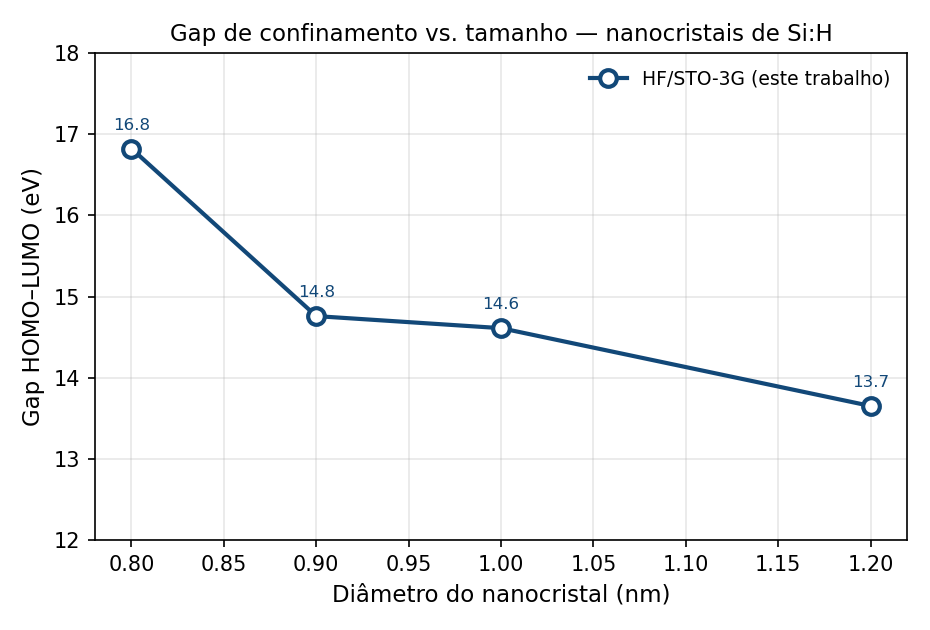
\includegraphics[width=0.78\textwidth]{figuras/gap_vs_tamanho.png}
  \caption{\emph{Gap} HOMO--LUMO calculado (HF/STO-3G) para nanocristais de Si:H
  em função do diâmetro. A queda monotônica com o tamanho é a assinatura do
  confinamento quântico. Os valores absolutos, porém, estão fortemente
  superestimados (ver texto).}
  \label{fig:gap}
\end{figure}

\begin{caixaatencao}
\textbf{A tendência é confiável; os valores absolutos, não.} Um leitor atento
estranhará: \emph{gaps} de $13$--$17$~eV? Nanocristais de Si desse tamanho exibem,
experimentalmente, \emph{gaps} ópticos de $3$--$4$~eV. Nosso cálculo os
superestima em cerca de quatro vezes --- e por bons motivos, todos instrutivos:
\begin{enumerate}[leftmargin=*,nosep]
  \item \textbf{Base mínima.} A STO-3G tem pouquíssimos orbitais virtuais, e eles
        ficam artificialmente altos, inflando o LUMO.
  \item \textbf{Ausência de correlação.} O Hartree-Fock ignora a correlação
        eletrônica e é notório por superestimar \emph{gaps}.
  \item \textbf{Orbitais virtuais de HF.} Os orbitais desocupados de HF sentem o
        potencial de $N$ elétrons (e não de $N-1$), o que os torna estimadores
        ruins de estados excitados.
\end{enumerate}
Isto não invalida o exercício --- pelo contrário. A \emph{física} (confinamento,
tendência com o tamanho) está correta; o que falha é a \emph{quantidade}. É
precisamente essa lacuna que motiva o Capítulo~5, onde a Teoria do Funcional da
Densidade e bases maiores nos aproximarão dos números experimentais.
\end{caixaatencao}

\subsection{O preço do realismo: o escalonamento na prática}

Ao rodar a varredura, você notará que os cálculos maiores demoram
desproporcionalmente mais. Na máquina em que este livro foi escrito, os tempos
foram: $\sim\!2$~s ($0{,}8$~nm, 106~funções), $17$~s ($0{,}9$~nm, 199), $27$~s
($1{,}0$~nm, 226) e $\sim\!8$~min ($1{,}2$~nm, 364). Quadruplicar o número de
funções de base multiplicou o tempo por mais de cem --- a assinatura do
escalonamento $N^4$ da Seção~\ref{sec:formalismo}. É por isso que o nanocristal
``oficial'' de $1{,}5$~nm (712~funções) do Projeto Âncora, embora perfeitamente
definível, exige paciência ou recursos de alto desempenho.

\begin{caixadica}
Para acelerar cálculos grandes, o \pyscf{} oferece o \emph{density fitting}, que
aproxima as integrais de dois elétrons e reduz drasticamente custo e memória:
\code{mf = scf.RHF(mol).density\_fit()}. O impacto na energia é pequeno; o ganho de
velocidade, enorme. Use-o sempre que o tamanho apertar.
\end{caixadica}

%---------------------------------------------------------------------
\begin{caixaancora}
\textbf{Etapa 1 --- O orbital do doador e o \emph{gap} eletrônico.}

Chegamos ao coração da Parte~I: localizar o \textbf{orbital que hospeda o
\qubit{}}. Diferentemente do silício puro (camada fechada), o sistema Si:P tem um
elétron desemparelhado. Num cálculo ROHF, isso se manifesta como um
\textbf{orbital simplesmente ocupado} (SOMO, \emph{Singly-Occupied Molecular
Orbital}): o estado do doador, com ocupação~1 em vez de~2 ou~0.

\vspace{0.2cm}
Por viabilidade computacional, executamos aqui o doador num nanocristal de
$1{,}0$~nm (Si$_{21}$P$_1$H$_{28}$, 337~elétrons); o de $1{,}5$~nm segue a mesma
receita, a custo maior.

\begin{lstlisting}[style=python]
import numpy as np
from pyscf import gto, scf
# reutiliza construir_nanocristal, inserir_doador, para_xyz do Capitulo 3

si, h = construir_nanocristal(1.0)
idx_p = inserir_doador(si)
mol = gto.M(atom=para_xyz(si, h, idx_p), basis='sto-3g', spin=1, verbose=0)

mf = scf.ROHF(mol)
mf.kernel()
assert mf.converged

# o SOMO e o orbital com ocupacao 1: o eletron do qubit
i_somo = int(np.where(mf.mo_occ == 1)[0][0])
print("SOMO: orbital #%d de %d, energia %.3f Ha"
      % (i_somo, len(mf.mo_occ), mf.mo_energy[i_somo]))

# quanto da densidade do SOMO esta localizada em torno do fosforo?
C = mf.mo_coeff[:, i_somo]
S = mol.intor('int1e_ovlp')
gross = C * (S @ C)                       # populacao por funcao de base
fatias = mol.aoslice_by_atom()
peso_atomo = np.array([gross[a[2]:a[3]].sum() for a in fatias])

iP = [mol.atom_symbol(i) for i in range(mol.natm)].index('P')
dist = np.linalg.norm(mol.atom_coords() - mol.atom_coords()[iP], axis=1) * 0.529
print("Densidade do SOMO sobre o P:        %.0f%%" % (100 * peso_atomo[iP]))
print("Densidade do SOMO ate 3 A do P:     %.0f%%" % (100 * peso_atomo[dist < 3].sum()))
\end{lstlisting}

\begin{lstlisting}[style=console]
SOMO: orbital #168 de 226, energia 0.157 Ha
Densidade do SOMO sobre o P:        19%
Densidade do SOMO ate 3 A do P:     83%
\end{lstlisting}

\textbf{O resultado que valida toda a Parte~I.} O orbital do \qubit{} não está
espalhado pelo nanocristal: \textbf{83\% de sua densidade concentra-se num raio de
$3$~Å em torno do fósforo}. O elétron excedente do doador está, de fato,
\emph{localizado} ao redor do P$^+$ --- é o ``hidrogênio artificial'' que a
intuição química do Capítulo~3 antecipou, agora confirmado por um cálculo de
primeiros princípios. É esse elétron localizado, e o seu spin, que
manipularemos como bit quântico.

\vspace{0.3cm}
\textbf{Sua tarefa.} No \emph{notebook} \code{projeto\_ancora\_SiP.ipynb}:
reproduza a varredura \emph{gap} vs.\ tamanho, gere a figura, e execute o cálculo
do doador acima. Registre: (a)~a energia do SOMO; (b)~o grau de localização;
(c)~por que a localização é essencial para um bom \qubit{} (dica: um estado
deslocalizado seria sensível a \emph{toda} a superfície e a suas imperfeições).

\vspace{0.3cm}
\textbf{A seguir.} No Capítulo~5, a Teoria do Funcional da Densidade corrigirá os
\emph{gaps} superestimados e nos dará acesso às propriedades ópticas do Si:P ---
antes de mergulharmos, na Parte~II, nos parâmetros magnéticos que definem o
\qubit{}: o acoplamento hiperfino e o tensor~\emph{g}.
\end{caixaancora}

%---------------------------------------------------------------------
\section*{Resumo do Capítulo}
\addcontentsline{toc}{section}{Resumo do Capítulo}
%---------------------------------------------------------------------

\begin{itemize}[leftmargin=*]
  \item O Hartree-Fock resolve as \textbf{equações de Roothaan-Hall}
        $\mathbf{FC} = \mathbf{SC}\boldsymbol{\varepsilon}$ de forma iterativa,
        porque a matriz de Fock depende da densidade que se quer obter --- o ciclo
        \textbf{SCF}.
  \item O custo escala como $N^4$ com o número de funções de base; por isso
        tamanho e base são sempre um compromisso, e o \emph{density fitting}
        (\code{.density\_fit()}) é um aliado valioso.
  \item A \textbf{convergência} é controlada por \emph{guess} inicial, DIIS,
        \code{level\_shift}, \code{max\_cycle} e \code{conv\_tol}. Sempre verifique
        \code{mf.converged} antes de usar resultados.
  \item O \textbf{gap} HOMO--LUMO de um ponto quântico é sua energia de
        confinamento: nossa varredura ($0{,}8$--$1{,}2$~nm) mostrou o \emph{gap}
        \textbf{diminuindo} com o tamanho, confirmando o confinamento quântico.
  \item Os valores absolutos de HF/STO-3G \textbf{superestimam} os \emph{gaps}
        (falta de correlação, base mínima, orbitais virtuais ruins) --- motivação
        para o DFT do Capítulo~5.
  \item \textbf{Projeto Âncora:} localizamos o \textbf{orbital do doador} (SOMO) no
        Si:P; \textbf{83\%} de sua densidade está a menos de $3$~Å do fósforo,
        confirmando o \qubit{} como um elétron localizado.
\end{itemize}

%---------------------------------------------------------------------
\section*{Exercícios}
\addcontentsline{toc}{section}{Exercícios}
%---------------------------------------------------------------------

\begin{enumerate}[leftmargin=*,label=\textbf{4.\arabic*}]
  \item \textbf{O ciclo SCF na prática.} Rode o nanocristal de $0{,}8$~nm com
        \code{verbose=4} e conte quantos ciclos o SCF levou para convergir. Depois
        aumente \code{mf.level\_shift} para $0{,}5$ e observe se o número de ciclos
        muda.

  \item \textbf{Verificando o escalonamento.} Cronometre (com o módulo \code{time})
        os cálculos de $0{,}8$, $0{,}9$ e $1{,}0$~nm. Faça um gráfico
        log--log do tempo contra \code{mol.nao} e estime o expoente do
        escalonamento. Ele se aproxima de~4?

  \item \textbf{Density fitting.} Repita o cálculo de $1{,}0$~nm com
        \code{scf.RHF(mol).density\_fit()} e compare energia total, \emph{gap} e
        tempo com o cálculo convencional. Valeu a pena?

  \item \textbf{Sensibilidade à base.} Recalcule o \emph{gap} do nanocristal de
        $0{,}8$~nm em STO-3G e em \code{6-31g}. O \emph{gap} sobe ou desce? Como
        isso se relaciona com a caixa de Atenção sobre valores absolutos?

  \item \textbf{O papel da passivação (revisão).} Construa o nanocristal de
        $0{,}8$~nm \emph{sem} passivar (sem hidrogênios) e tente rodar o SCF. Você
        provavelmente terá dificuldade de convergência ou um \emph{gap}
        minúsculo. Explique, com base nas ligações pendentes do Capítulo~3, o que
        aconteceu.

  \item \textbf{Projeto Âncora.} Para o doador Si:P de $1{,}0$~nm, examine também o
        orbital duplamente ocupado logo abaixo do SOMO e o primeiro virtual acima.
        Eles estão localizados no fósforo ou espalhados pelo nanocristal? O que
        isso diz sobre a natureza especial do estado do doador?
\end{enumerate}
